\documentclass[preview]{standalone}

\usepackage{amsmath}
\usepackage{amssymb}
\usepackage{stellar}
\usepackage{bettelini}

\hypersetup{
    colorlinks=true,
    linkcolor=black,
    urlcolor=blue,
    pdftitle={Biologia},
    pdfpagemode=FullScreen,
}

\begin{document}

\title{Biologia}
\id{biologia-genetica-molecolare}
\genpage

% TODO: Deossiribosio e ribosio

\begin{snippet}{e13a1dac-ac32-465b-bfca-22400f749c91}
    Le basi azotate del DNA possono essere quattro:
    \textbf{adenina} (A),
    \textbf{timina} (T),
    \textbf{citosina} (C) e
    \textbf{guanina} (G).
    Nell'RNA, invece, abbiamo la \textbf{uracile} (U) al posto della timina.

    L'RNA è caratterizzato da un singolo filamento di nucleotidi,
    mentre il DNA da due catene di nucleotidi.
    Nell'RNA lo zucchero è il ribosio.

    % immagini delle basi azotate

    Le basi azotate sono complementari e formano di ponti idrogeno
    fra una molecola e l'altro.
    La A si lega sempre con la T e la G con la C.
    Nell'RNA la U non si lega perché è un unico filamento.
    Entrambi hanno una conformazione tridimensionale ad elica
    (doppia nel DNA e singola nell'RNA).
\end{snippet}

\begin{snippet}{xna-illustration}
    \begin{center}
    \begin{figure}[th]
        \centering
        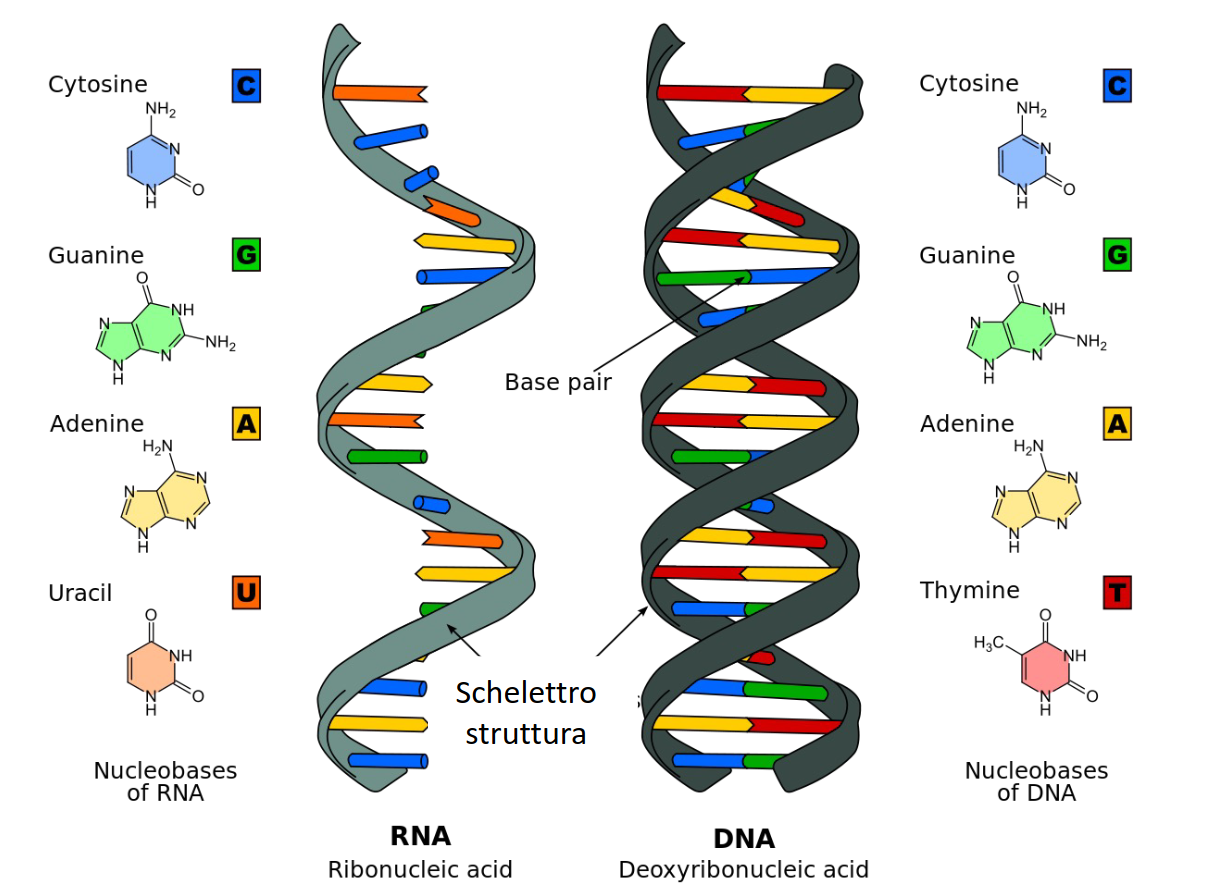
\includegraphics[width=\textwidth]{./resources/xna.png}
    \end{figure}
    \end{center}
\end{snippet}

\begin{snippet}{bd4fb6c3-0d4c-4e1f-a160-fb3fb5811a1d}
    I due filamenti di DNA sono anti-paralleli nel senso
    che uno va nel senso dell'altro.

    Il DNA possiede una doppia elica perché è una molecola
    più stabile e più difficile da rompere.
    Quando una catena di DNA si duplica, un enzima
    inserisce le basi complementari corrispondenti.
    In caso di errore un enzima se ne accorge e viene corretto.
\end{snippet}

\end{document}